\chapter{Data structure}\label{ch:data-structure}

\section{Skiplist is suitable for range lock}
The effectiveness of a range lock is strongly influenced by the underlying data structure used to manage these ranges. 
Existing range locks have used many different comparison-based data structures, such as interval tree~\parencite{linuxRangeLockImpl2013, kim2019pnova} and linked list~\parencite{song2013parallelizing}, skip list~\parencite{kogan2020scalable} each of which has advantages and disadvantages. 

Interval trees are considered heavyweight compared to linked lists and skip lists because they require complex balancing mechanisms to maintain efficient search times, which adds significant computational and memory overhead. 
Interval trees also require the maintenance of additional data, such as subtree intervals, making them more resource-intensive. This makes interval trees unsuitable for range locking. 

Linked lists have minimal structure and are easy to implement and maintain. However, it is very expensive in terms of Insert/Delete time. The complexity O(n) for the average case of search becomes a significant disadvantage when the number of ranges increases, 

Skiplists strike a balance between the heaviness of interval trees and the simplicity of linked lists. Despite their theoretically poor worst-case performance, skip lists rarely exhibit worst-case behavior, making them efficient in most scenarios.
For example, in a dictionary with more than 250 entries, the probability that a search will take more than three times the expected time is less than one in a million~\parencite{pugh1990skip2}. 

We strongly believe that the skip list is ideal for implementing range locking.

\begin{table}[h!]
    \centering
    \begin{tabular}{|c|c|c|c|}
        \hline
        \textbf{Data Structure} & \textbf{Best Case} & \textbf{Average Case} & \textbf{Worst Case} \\ \hline
        \textbf{Linked List} & $O(1)$ & $O(n)$ & $O(n)$ \\ \hline
        \textbf{Skip List} & $O(1)$ & $O(logn)$ & $O(n)$ \\ \hline
        \textbf{Interval Tree} & $O(\log n)$ & $O(\log n)$ & $O(\log n)$ \\ \hline
    \end{tabular}
    \caption{Time complexities of Insert/Delete operations in Linked List, Skip List and Interval Tree}
    \label{tab:insertdeletecomplexity}
\end{table}

\begin{figure}[h!]
    \centering
    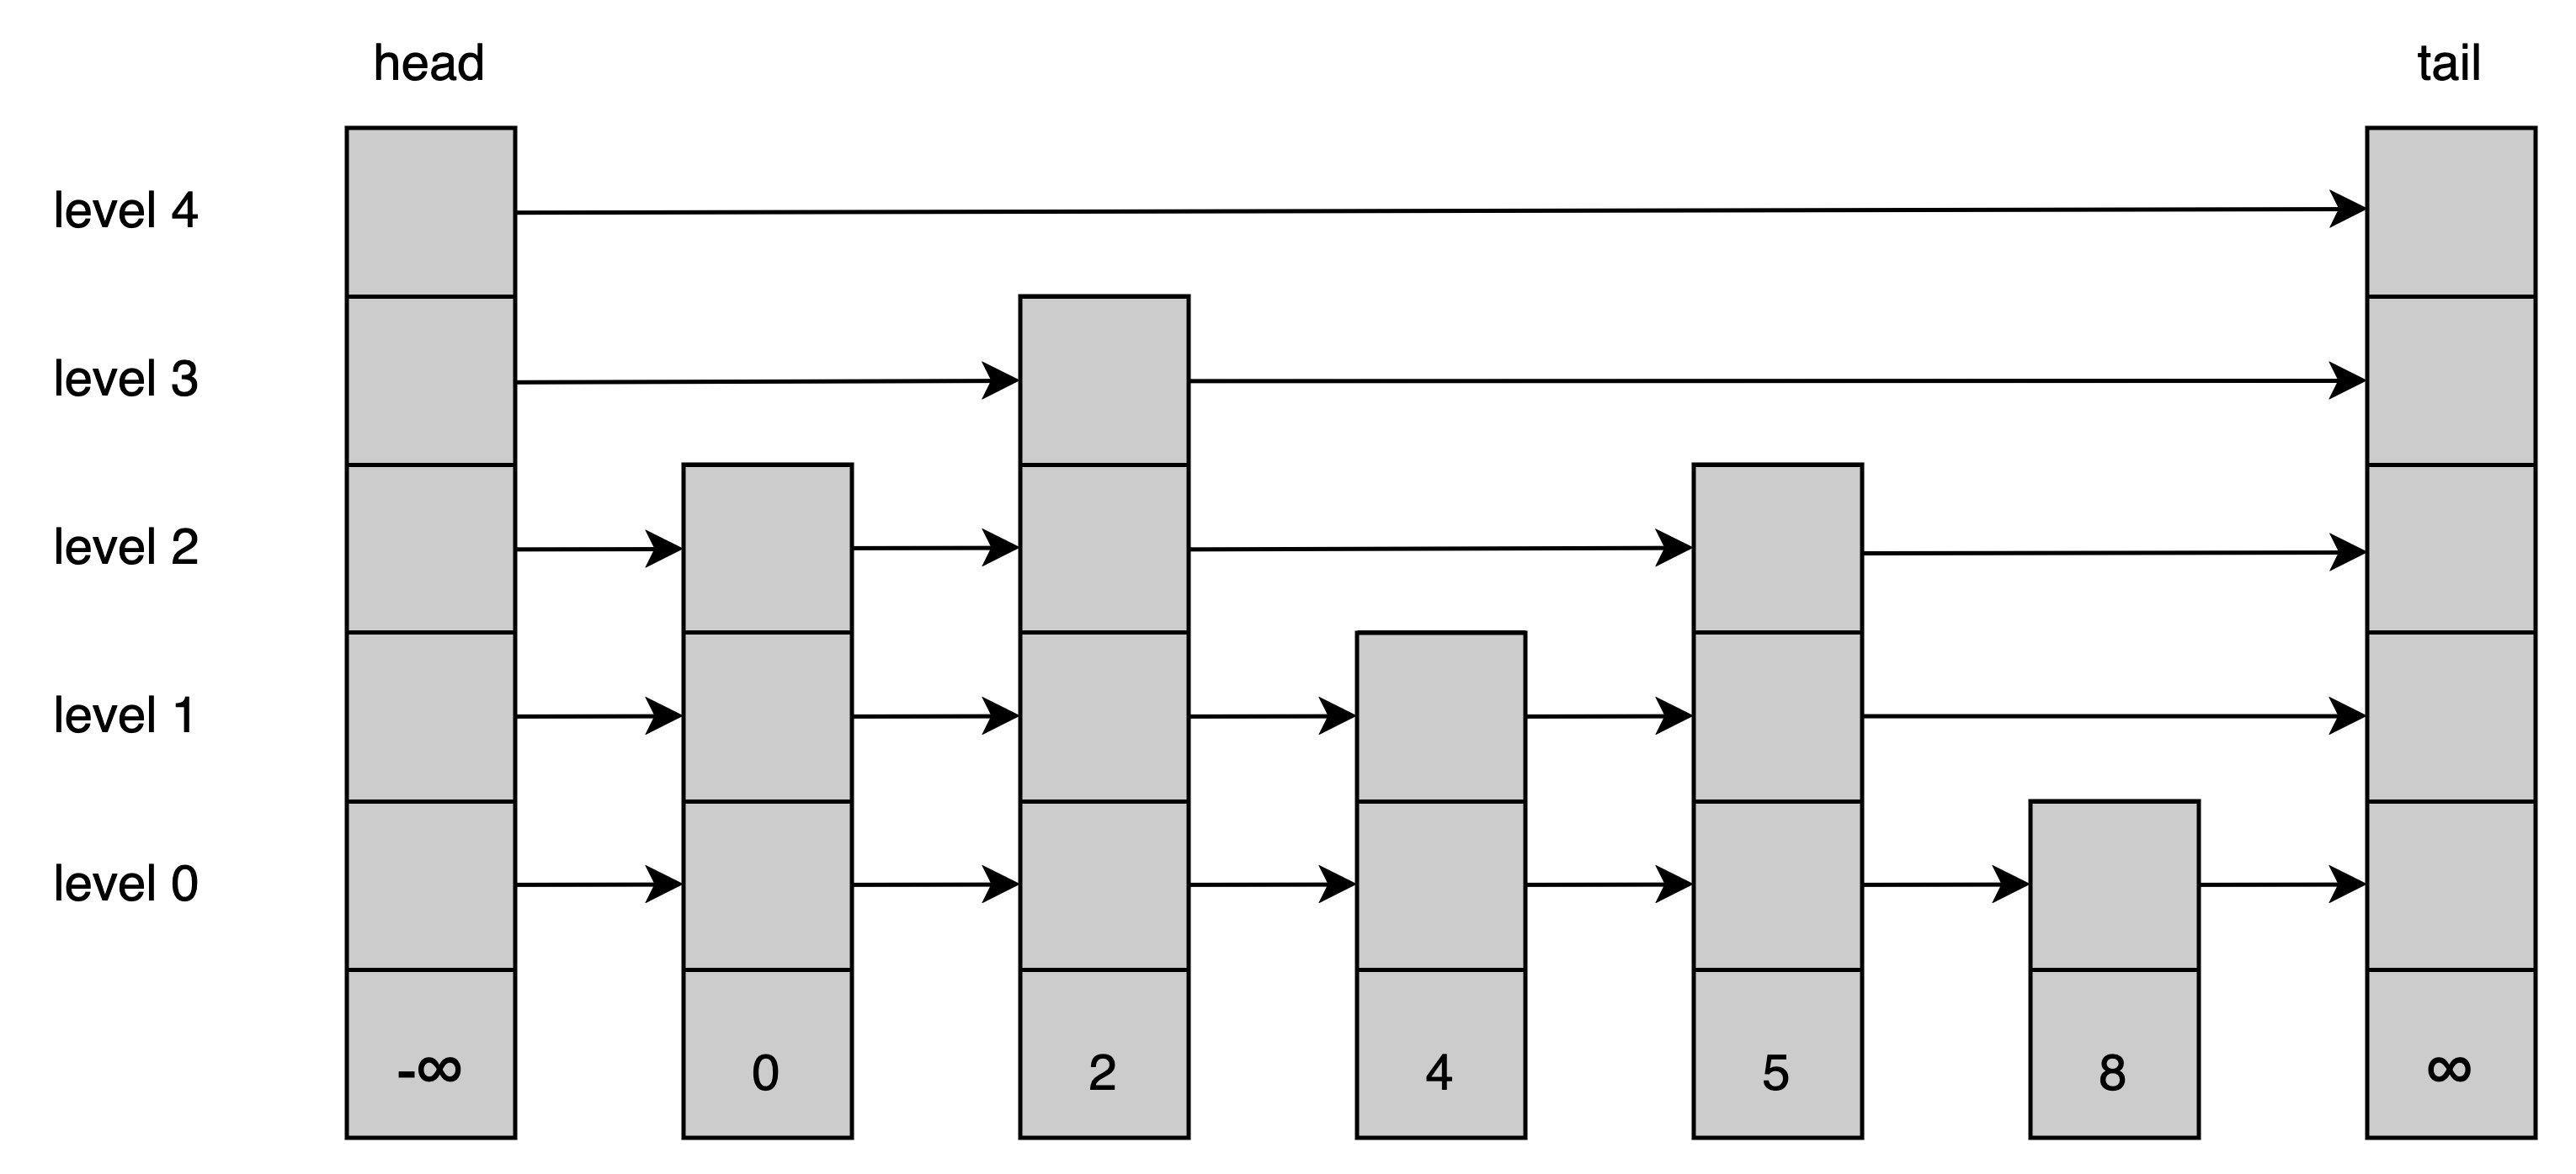
\includegraphics[width=0.8\textwidth]{./figures/skiplist.png}
    \caption{An example of a skip list. It has five levels of sorted linked lists.}
    \label{fig:skiplist}
\end{figure}

\section{Modification of skiplist for concurrent range lock}

We developed our concurrent range lock based on the \texttt{LockFreeSkipList} proposed by Herlihy et al.~\parencite{herlihy2020art}.
In summary, \texttt{LockFreeSkipList} uses atomic operations (\texttt{compareAndSet()}) to manage node references without locks, which enhances performance in multithreaded environments.
When adding a node, the process starts at the lowest level and moves upward to ensure immediate visibility.
Removing a node involves marking nodes from the top down before unlinking them.
Furthermore, it relaxes strict structural maintenance of higher levels, focusing on the bottom-level list for set representation, which offers improved scalability and efficiency.

However, conventional skiplists does not work out of the box for range locking. Firstly, each node of the skiplist stores key and value, not range. Secondly, the comparison condition needs to be modified because we now must compare both range start and range end while inserting or deleting instead of just using the key. We present this in two critical changes in the Sections \ref{subsec:node} and \ref{subsec:find}, respectively.

\subsection{Node}\label{subsec:node}

\texttt{Node} is the base of our \texttt{ConcurrentRangeLock} structure.
Each \texttt{Node} instance now contains \textbf{\texttt{start}} and \textbf{\texttt{end}}, which represent one range.
\texttt{Node} uses an array of \textbf{\texttt{AtomicMarkableReference}} (more details in Section \ref{subsec:atomicmarkablereference}) to maintain forward links at each level, which allows for efficient traversal and updates. 
\texttt{Node} provides the following methods:

\begin{itemize}
    \item \texttt{initialize}: sets up a node with specific range and level values.
    \item \textbf{\texttt{initializeHead}}: configures the head node with forward pointers directed to a provided tail node, establishing the initial structure.
    \item \texttt{getTopLevel()}, \texttt{getStart()}, \texttt{getEnd()}: accessor methods to retrieve the properties of node.
\end{itemize}

\begin{figure}[h]
    \centering
    \lstinputlisting[style=mystyle,caption={\texttt{ConcurrentRangeLock}: \texttt{Node} class},label={lst:node}]{code/node.txt}
\end{figure}

\clearpage

\subsection{AtomicMarkableReference} \label{subsec:atomicmarkablereference}

\texttt{Node} use an array of \texttt{AtomicMarkableReference} to maintain the express layer. 
An \texttt{AtomicMarkableReference} object encapsulates both a reference to an object of type T and a Boolean mark. 
These fields can be atomically updated, either together or individually. 
The  class uses a single atomic variable, \texttt{atomicRefMark}, to store a packed representation of both the reference and a mark. 
If the mark is \texttt{1}, it indicates that the node references to it is softly deleted. 
These values are packed and unpacked using bitwise operations, where the least significant bit represents the mark.

Listing \ref{lst:atomicmarkablereference} provides the algorithm for \texttt{AtomicMarkableReference}.

The \texttt{pack} method combines a node pointer and a boolean mark into a single \texttt{uintptr\_t} value by encoding the pointer into the lower bits and the mark into the highest bit. Conversely, the \texttt{unpack} method decodes this packed value to retrieve the original node pointer and boolean mark.

To atomically set a new node pointer and mark value, the \texttt{store} method uses relaxed memory ordering.

The \texttt{compareAndSet} method performs an atomic update of both the reference and mark if they match the expected values, employing acquire-release memory ordering for proper synchronization.

The \texttt{attemptMark} method focuses on updating the mark alone, provided that the current reference matches the expected one and the mark differs. If the update succeeds, it returns \texttt{true}; otherwise, it returns \texttt{false}.

The \texttt{get} method retrieves the current reference and mark, which stores the mark in a provided boolean pointer. In contrast, the \texttt{getReference} method returns the current reference without accessing the mark.

\begin{figure}[!p]
    \centering
    \lstinputlisting[style=mystyle,caption={\texttt{ConcurrentRangeLock}: \texttt{AtomicMarkableReference} class.},label={lst:atomicmarkablereference}]{code/atomicmarkablereference.txt}
\end{figure}